\documentclass[english]{article}

\usepackage[latin9]{inputenc}
\usepackage[letterpaper]{geometry}
\geometry{verbose,tmargin=1in,bmargin=1in,lmargin=1in,rmargin=1in}
\usepackage{amsmath}
\usepackage{amssymb}
\usepackage{graphicx}
\usepackage{float}
\restylefloat{table}

\title{CIS 520, Machine Learning, Fall 2015: Assignment 4 \\
Due: Thursday, October 15th, 11:59pm, PDF to Canvas\\}
\date{}
\author{Arpit Panwar}

\begin{document}
\maketitle

\section*{Boosting and MDL}
\label{sec:boosting}

\subsection*{1. Analyzing the training error of boosting}

Consider the AdaBoost algorithm you saw in class. In this question
we will try to analyze the training error of boosting.

\begin{enumerate}
\item Given a set of $m$ examples, $(x_i,y_i)$ ($y_i$ is
  the class label of $x_i$), $i=1,\ldots,m$, let $h_t(x)$ be the weak
  classifier obtained at step $t$, and let $\alpha_t$ be its
  weight. Recall that the final classifier is
  \[
  H(x) = \mbox{sign} (f(x)), \mbox{ where } f(x) = \sum_{t=1}^T
  \alpha_t h_t(x).
  \]
  Show that the training error of the final classifier can be bounded
  from above by an exponential loss function:
  \[
  \frac{1}{m} \sum_{i=1}^m I(H(x_i) \neq y_i) \leq \frac{1}{m}
  \sum_{i=1}^m \exp( -f(x_i) y_i),
  \]
  where $I(a=b)$ is the indicator function. It is equal to 1 if $a=b$,
  and 0 otherwise

  {\em Hint}: $e^{-x} \geq 1 \Leftrightarrow x \leq 0$. 

\begin{align*}
	D_{t+1}(i) =&\; \dfrac{D_{t-1}(i) * e ^{-\alpha_t * y_i * h_t(x_i)} * e^{-\alpha_{t-1} * y_{i} * h_{t-1}(x_i)}}
				{Z_t * Z_{t-1}} \\
	&\;Expanding \; till \; D_1 \\
	=&\;\dfrac{D_1(i) *  e^ {-\alpha_t * y_i * h_t (x_i) } * e^{-\alpha_{t-1}*y_i*h_{t-1}(x_i)} \ldots e^{-\alpha_1 * y_i * h_1{x_i}}}
		       {Z_t * Z_{t-1} * Z_{t-1} \ldots * Z_1} \\
	=&\; \dfrac{e^{\sum_t {y_t * \alpha_t * h_t(x_i)}}}
		        {m * \prod_t{Z_t}} \\
	D_{t+1}(i) =&\; \dfrac {e^{-y_i f(x_i)}} {m * \prod_t Z_t} \\
	&\;When \; H(x_i) \neq y_i \; y_i * f(x_i) \leq 0. \; Thus \; e^{-y_i*f(x_i)} \geq 1\\
	&\;I(H(x_i) \neq y_i) \leq e^{-y_i*f(x_i)} \\
	&\;\frac{1}{m} * \sum_i {I(H(x_i) \neq y_i)} = \frac{1}{m} * \sum_i {e^{-y_i*f(x_i)}}\\
\end{align*}


\item 
  Remember that
  \[D_{t+1}(i)=\frac{D_t(i)\exp(-\alpha_ty_ih_t(x_i))}{Z_t}\] Use this
  recursive definition to prove the following.
  \begin{equation}
    \label{boosting:upper bound} \frac{1}{m} \sum_{i=1}^m \exp( -f(x_i)
    y_i) = \prod_{t=1}^T Z_t,
  \end{equation}
  where $Z_t$ is the normalization factor for distribution $D_{t+1}$:
  \begin{equation}
    \label{boosting:normalization_expression} Z_t = \sum_{i=1}^m D_t(i)
    \exp(-\alpha_t y_i h_t(x_i)).
  \end{equation}

  {\em Hint}: Remember that $e^{\sum_i g_i}=\prod_i
  e^{g_i}$,$D_1(i)=\frac{1}{m}$, and that $\sum_i D_{t+1}(i) = 1$.

\begin{align*}
	&\;Expanding\; the\; above\; equation \; for \; D_{t+1} \\
	D_{t+1}(i) =&\; \dfrac{D_{t-1}(i) * e ^{-\alpha_t * y_i * h_t(x_i)} * e^{-\alpha_{t-1} * y_{i} * h_{t-1}(x_i)}}
				{Z_t * Z_{t-1}} \\
	&\;Expanding \; till \; D_1 \\
	=&\;\dfrac{D_1(i) *  e^ {-\alpha_t * y_i * h_t (x_i) } * e^{-\alpha_{t-1}*y_i*h_{t-1}(x_i)} \ldots e^{-\alpha_1 * y_i * h_1{x_i}}}
		       {Z_t * Z_{t-1} * Z_{t-1} \ldots * Z_1} \\
	=&\; \dfrac{e^{\sum_t {y_t * \alpha_t * h_t(x_i)}}}
		        {m * \prod_t{Z_t}} \\
	=&\;\dfrac{e^{-y_i \sum_t{\alpha_t h_t()x_i}}}
		      {m * \prod_t{Z_t}} \\
	&\;We \; know\; that f(x) = \sum_t {\alpha_t * h_t(x_i)} \\
	D_{t+1}(i) =&\; \dfrac {e^{-y_i f(x_i)}} {m * \prod_t Z_t} \\
	&\;Summing\; over\; all \; i \\
	\sum_i {D_{t+1}(i)} =&\; \dfrac {\sum_i {e^{-y_i * f(x_i)}}} {m * \prod_t {Z_t}} \\
	&\;We \; know \; \sum_i {D_{t+1}(i)} = 1 . Substituting \; and \; rearranging \\
	 \prod_t {Z_t} = &\; \sum_i {e^{-y_i * f(x_i)}} \\
\end{align*}


\item  \begin{equation} \frac{1}{m} \sum_{i=1}^m \exp( -f(x_i)
    y_i) = \prod_{t=1}^T Z_t,
  \end{equation}
 suggests that the
  training error can be reduced rapidly by greedily optimizing $Z_t$
  at each step.  You have shown that the error is bounded from above:
  \[
  \epsilon_{training} \leq \prod_{t=1}^T Z_t.
  \]
  Observe that $Z_1, \dots, Z_{t-1}$ are determined by the first
  $(t-1)$ rounds of boosting, and we cannot change them on round $t$.
  A greedy step we can take to minimize the training error bound on
  round $t$ is to minimize $Z_t$.

  In this question, you will prove that for binary weak classifiers,
  $Z_t$ from 
\begin{equation}
    \label{boosting:normalization_expression} Z_t = \sum_{i=1}^m D_t(i)
    \exp(-\alpha_t y_i h_t(x_i)).
  \end{equation}
 is minimized by picking $\alpha_t$ as:
  \begin{equation}\label{eq:alpha}
    \alpha_t^* = \frac{1}{2}\log\left( \frac{1 - \epsilon_t}{\epsilon_t}
    \right),
  \end{equation}
  where $\epsilon_t$ is the training error of weak classifier $h_t$
  for the weighted dataset:
  \[
  \epsilon_t = \sum_{i=1}^m D_{t}(i) I(h_t(x_i) \neq y_i).
  \]
  where $I$ is the indicator function. For this proof, only consider
  the simplest case of binary classifiers, i.e. the output of $h_t(x)$
  is binary, \{$-1,+1$\}.

  For this special class of classifiers, first show that the
  normalizer $Z_t$ can be written as:
  \[
  Z_t = (1-\epsilon_t)\exp(-\alpha_t) + \epsilon_t\exp(\alpha_t).
  \]

  {\em Hint}: Consider the sums over correctly and incorrectly
  classified examples separately.
\begin{align*}
	 Z_t =&\; \sum_{i=1}^m D_t(i) \exp(-\alpha_t y_i h_t(x_i)) \\
	&\;Splitting\; into \; with \; h(x_i) \neq y_i \; and \; h(x_i) = y_i \\
	Z_t =&\; \sum_{ h(x_i) = y_i} {D_t(x_i) e^{-y_i * \alpha_i * h_t(x_i)}} + \sum_{ h(x_i) \neq y_i} {D_t(x_i) e^{-y_i * \alpha_i * h_t(x_i)}} \\
	&\;We \;know \;that \;   \epsilon_t = \sum_{i=1}^m D_{t}(i) I(h_t(x_i) \neq y_i). \\
	&\;Additionally \; we \; know \; e^{-y_i*\alpha_t * h_t (x_i)} = e^{-\alpha_t} \; when h_t(x_i) = y_i  and e^{-y_i*\alpha_t * h_t (x_i)} =  \\
	&\; Also \; since \; the \; classifier \; is \; binary \; we \; when \; we \; classify \; correctly \; the \; error \; is \; (1 - \epsilon_t) \\
	Z_t =&\; (1 - \epsilon_t) e^{-\alpha_t} + \epsilon_t e^{\alpha_t} \\ 
\end{align*}


\item  Now, prove that the value of $\alpha_t$ that
  minimizes this definition of $Z_t$ is given by Equation
 \begin{equation}
    \alpha_t^* = \frac{1}{2}\log\left( \frac{1 - \epsilon_t}{\epsilon_t}
    \right).
  \end{equation}

\begin{align*}
	&\; Using \; the \; equation \; above \; and \; taking \; differential \; w.r.t \; \alpha_t  \; and \; setting \; to \; 0\\
	\frac{d{Z_t}}{d{\alpha_t}} = &\; \frac{d}{d{\alpha_t}} (1 - \epsilon_t) e^{-\alpha_t} + \frac{d}{d{\alpha_t}} \epsilon_t * e^{-\alpha_t} \\
	 0 =&\; - (1 - \epsilon_t) e^{-\alpha_t} + \epsilon_t e^{\alpha_t} \\
	 \epsilon_t e^{\alpha_t} =&\; (1 - \epsilon_t) e^{-\alpha_t} \\
	e^{\alpha_t} =&\; \dfrac{(1 - \epsilon_t) * e ^ {-\alpha_t}} {\epsilon_t} \\
	e^{2 \alpha_t} =&\; \dfrac{1-\epsilon_t}{\epsilon_t} \\
	2 \alpha_t =&\; \log {\dfrac{1-\epsilon_t}{\epsilon_t}} \\
	\alpha_t =&\; \frac{1}{2} * \log {\dfrac{1-\epsilon_t}{\epsilon_t}}
\end{align*}

\item Prove that for the above value of $\alpha_t$ we
  have $Z_t = 2\sqrt{\epsilon_t(1-\epsilon_t)}$.

Substituting the values from 1.3 into 1.4 \\
\begin{align*}
	Z_t = &\; \dfrac{1 - \epsilon_t}{ \sqrt{\dfrac{1 - \epsilon_t}{\epsilon_t}}} + \epsilon_t * \sqrt {\dfrac {1 - \epsilon_t}{\epsilon_t} } \\
	=&\; \dfrac{1 - \epsilon_t} {\sqrt {\dfrac{1 - \epsilon_t} {\epsilon_t}} } + \sqrt {\epsilon_t * (1 - \epsilon_t)} \\
	=&\; \sqrt {\epsilon_t * (1 - \epsilon_t)} + \sqrt {\epsilon_t * (1 - \epsilon_t)} \\
	=&\; 2 * \sqrt {\epsilon_t * (1 - \epsilon_t)} \\
\end{align*}


\item Furthermore, let $\epsilon_t=\frac{1}{2}-\gamma_t$
  and prove that $Z_t\leq \exp(-2\gamma_t^2)$.  Therefore, we will
  know
  \begin{equation*}
    \epsilon_{training} \le \prod_tZ_t \le
    \exp(-2\sum_t\gamma_t^2).
  \end{equation*}

  {\em Hint}: $\log(1-x)\leq -x$ for $0<x\leq 1$.

Using 1.5  and substituting the value for $\epsilon_t$ \\
\begin{align*}
	Z_t =&\; 2 \sqrt{ (\frac{1}{2} - \gamma_t) * (1 - \frac{1}{2} + \gamma_t)} \\
	=&\; 2 \sqrt {\frac{1}{4} - \gamma_t^2} \\
	=&\; \sqrt{1 - 4 \gamma_t^2} \\
	=&\; e^{ \frac{1}{2} \log{1 - 4 \gamma_t^2}} \\
	&\;Using \;  \log(1-x)\leq -x \\
	Z_t \leq &\; e^{\frac{1}{2} * 4 * - \gamma_t^2} \\
	Z_t \leq &\; e^{-2 \gamma_t^2 } \\
	\prod_t Z_t \leq &\; e^{\sum_t -2 \gamma_t^2} \\
\end{align*}

\item For every step of AdaBoost in a binary classifier if we have a classifier with $\epsilon_t >0.5$ then there will always be a classifier which classifies exactly opposite and has an error $1 - \epsilon_t$.\\
Additionally if $\epsilon_t > 0.5$ we get $\alpha_t < 0$ which will penalize the correct prediction and not the once predicted incorrectly. And since we know that we always converge the weak classifier should have error $<$ 0.5.


\item For $\epsilon_t = 0.5$ , using the equation for $\alpha_t$ above, we get $alpha_t = 0$. Thus $D_{t+1} = D_t$ thus the error gets stuck.
\end{enumerate}

\subsection*{2. Adaboost on a toy dataset}

\begin{figure}[t]
  \begin{center}
    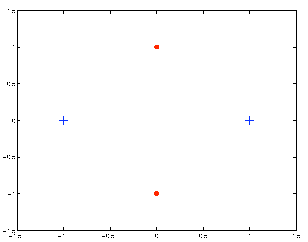
\includegraphics[width=2in]{images/toydata}
    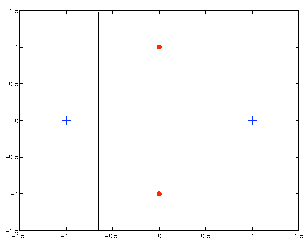
\includegraphics[width=2in]{images/toydata_with_h1}
  \end{center}
  \caption{a) Toy data in Question~\ref{sec:boosting}. b) $h_1$ in Question~\ref{sec:boosting}}
  \label{fig:toydata}
\end{figure}

Now we will apply Adaboost to classify a toy dataset. Consider the
dataset shown in Figure~\ref{fig:toydata}a. The dataset consists of
$4$ points: ($X_1 : 0,-1,-$), ($X_2 : 1,0,+$), ($X_3 : -1,0,+$) and
($X_4 : 0,1,-$).  For this part, you may find it helpful to use MATLAB
as a calculator rather than doing the computations by hand.  (You do
not need to submit any code though.)

\begin{enumerate}
\item  For $T=4$, show how Adaboost works for this dataset,
  using simple decision stumps (depth-1 decision trees that simply
  split on a single variable once) as weak classifiers.  For each
  timestep compute the following:
  \[ \epsilon_t, \alpha_t, Z_t, D_t(i)~\forall i, \] Also for each
  timestep draw your weak classifier. For example $h_1$ can be as
  shown in ~\ref{fig:toydata}b). 

\begin{table}[H]
\centering
\caption{Errors and Alphas}
\label{Values}
\begin{tabular}{|l|l|l|l|l|}
\hline
      & T=1                       & T=2                                     & T=3                         & T=4                                    \\ \hline
E     & 0.2500                    & 0.1667                                  & 0.1000                      & 0.0556                                 \\ \hline
Alpha & 0.5493                    & 0.8047                                  & 1.0986                      & 1.4166                                 \\ \hline
D     & {[}0.25;0.25;0.25;0.25{]} & {[}0.1667 ; 0.1667 ; 0.5000 ; 0.1667{]} & {[}0.1 ; 0.1 ; 0.3 ; 0.5{]} & {[}0.0556 ; 0.500 ; 0.1667 ; 0.2778{]} \\ \hline
Z     & 0.8660                    & 0.7454                                  & 0.6000                      & 0.4581                                 \\ \hline
\end{tabular}
\end{table}

\begin{figure}[t]
 \begin{center}
    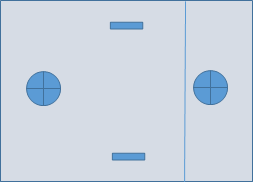
\includegraphics[width=2in]{images/2_1_1}
    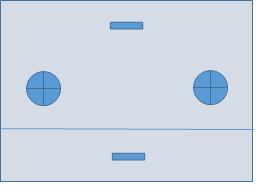
\includegraphics[width=2in]{images/2_1_2}
    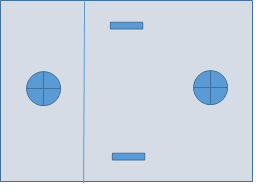
\includegraphics[width=2in]{images/2_1_3}
    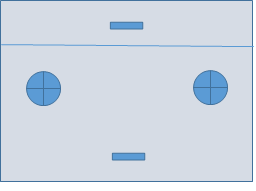
\includegraphics[width=2in]{images/2_1_4}
  \end{center}
  \caption{a) H1 ~\ref{sec:boosting} b) H2 ~\ref{sec:boosting} c) H3 ~\ref{sec:boosting} d) H4 ~\ref{sec:boosting} }
\end{figure}

\item 
Training error is 0


\item 
 The dataset is not linearly separable. Since the dataset is not linearly separable, decision tree can not make a better decision on non-linear dataset.

  %% Don't remove the empty line below.  Compilation will fail.

\end{enumerate}



\subsection*{3. MDL on a toy dataset}

Consider the following problem

 We provide a data set generated from a particular model with $N=64$.

where we want to estimate

\begin{equation*}
 \hat{y} =  w_1 x_1 + w_2 x_2 + w_3 x_3 
\end{equation*}

We want to use MDL to find the 'optimal' $L_0$-penalized model.

\begin{enumerate}
\item  Estimate the three linear regressions \\

(We could actually try all possible subsets here, but instead we'll just try three.)

\begin{align*}
  y_1& = w_1 x_1 \\
  y_2& = w_1 x_1 + w_2 x_2 \\
  y_3& = w_1 x_1 + w_2 x_2 + w_3 x_3  \\
\end{align*}

For each of the three cases, what is
\begin{enumerate}
\item the sum of square error \\
i)   $\text{Err}_1 = 1.2779e+03 $ \\
ii)  $\text{Err}_2 =  835.0558$\\
iii) $\text{Err}_3 = 834.7418$\\

\item 2 times the estimated bits to code the residual ($n \log{\frac{Error}{n}} $)  \\
i)    $\text{ERR}\_\text{bits}_1 = 191.6237 $ \\
ii)   $\text{ERR}\_\text{bits}_2 = 164.3914$ \\
iii)  $\text{ERR}\_\text{bits}_3 = 164.3973$ \\

\item 2 times the estimated bits to code each residual plus model under AIC ($2*1$ bit to code each feature) \\
i)    $\text{AIC}\_\text{bits}_1 = 193.6237$ \\
ii)   $\text{AIC}\_\text{bits}_2 = 168.3914$ \\
iii)  $\text{AIC}\_\text{bits}_3 = 170.3673$ \\

\item 2 times the estimated bits to code each residual plus model under BIC  ($2*(1/2) log(n)$ bits to code each feature) \\
i)   $\text{BIC}\_\text{bits}_1 = 195.7826$ \\
ii)  $\text{BIC}\_\text{bits}_2 = 172.7092$ \\
iii) $\text{BIC}\_\text{bits}_3 = 176.8440$ \\

\end{enumerate}

\item Which model has the smallest minimum description length? \\
a) for AIC :- Model 2 gives minimum MDL\\
b) for BIC :- Model 2 gives minimum MDL\\

\item  
i. Error for model 1 = $1.7786e+03$ \\
ii. Error for model 2 = $1.1671e+03$ \\
iii. Error for model 3 = $1.1727e+03$ \\

\end{enumerate}


\end{document}
